\documentclass{article}

\usepackage{amsmath}
\usepackage{fancyhdr}
\usepackage{graphicx}
\graphicspath{{}}

%% some colours
\usepackage{color}
\definecolor{deepblue}{rgb}{0,0,0.5}
\definecolor{deepred}{rgb}{0.6,0,0}
\definecolor{deepgreen}{rgb}{0,0.5,0}
\definecolor{backcolour}{rgb}{0.95,0.96,0.93}

%%%%%%%%%%%%%% CODE STUFF %%%%%%%%%%%%%%
%%%%%%%%%%%%%%%%%%%%%%%%%%%%%%%%%%%%%%%%
\usepackage{cprotect} % to be used in sol
\usepackage{listings} % for code display
% setting code style
\newcommand\pythonstyle{\lstset{
        language=Python,
        backgroundcolor=\color{backcolour},
		basicstyle=\footnotesize,
		otherkeywords={self},
		keywordstyle=\footnotesize\color{deepblue},
		emph={__init__},
		emphstyle=\footnotesize\color{deepred},
		stringstyle=\color{deepgreen},
		frame=single,
		showstringspaces=false  ,
		breaklines=true,
		numbers=left,
		numberstyle=\footnotesize,
		tabsize=4,
		breakatwhitespace=false
	}}

% Python environment
\lstnewenvironment{python}[1][]{
    \pythonstyle
    \lstset{#1}
}{}

% Python for external files
\newcommand\pythonexternal[2][]{{
    \pythonstyle
    \lstinputlisting[#1]{#2}
}}

% Python for inline
\newcommand\pythoninline[1]{{\pythonstyle\lstinline!#1!}}

%%%%%%%%%%%%%%%%%%%%%%%%%%%%%%%%%%%%%%%%
% setting the style for ex documents
\pagestyle{fancy}
\fancyhf{}
\fancyhead[L]{\thetitle}
\fancyhead[C]{}
\fancyhead[R]{\theauthor}
\renewcommand{\headrulewidth}{0.4pt} %obere Trennlinie
\fancyfoot[L]{Due: \thedate}
\fancyfoot[R]{\thepage} %Seitennummer
\renewcommand{\footrulewidth}{0.4pt}

% include solutions
\newcommand\sol[1]{{\large\textbf{\\Solution:}}#1}
\usepackage{tikz}
\usetikzlibrary{arrows,automata}

\title{BPP Exercise 5 - Strings and RegEx}
\author{A. Hain, M. Nipshagen}
\date{07.05.2018, 18:00}

\makeatletter
\let\thetitle\@title
\let\theauthor\@author
\let\thedate\@date
\makeatother

% do not include solutions
% \renewcommand\sol[1]{}


\begin{document}

The deadline for this exercise sheet is \textbf{Monday, \thedate.}
%
%\section*{Introductory Words}
%In case we have some information that doesn't directly concern the current exercises.
%

\section{Warm-Up: Regular Expressions}
For each of these RegEx, please indicate which of the given statements can be described by the RegEx.\\
For each of the statements that \textit{cannot} be described by the given RegEx, please explain, why.

\subsection{}
Can these statements be described by this RegEx: \textbf{ab?c+}
\begin{itemize}
\item[a)] abc \sol{Yes.}
\item[b)] ab \sol{No. There needs to be at least one c.}
\item[c)] abcc \sol{Yes.}
\item[d)] accc \sol{Yes.}
\end{itemize}

\subsection{}
Can these statements be described by this RegEx: \textbf{\string^((xy)\textbar[0-9]*)*\$}
\begin{itemize}
\item[a)] 159yx1 \sol{No. It needs to be xy, not yx.}
\item[b)] xyxyxyxy1 \sol{Yes.}
\item[c)] 1xy27xy385 \sol{Yes.}
\item[d)] 12345xy67ab89 \sol{No. This RegEx does not include the characters a or b.}
\end{itemize}

\subsection{}
Can these statements be described by this RegEx: \textbf{(x*)(.[a-k])y\textbackslash2\textbackslash1}
\begin{itemize}
\item[a)] xxxyayyaxxx \sol{Yes.}
\item[b)] xx0my0mxx \sol{No. Group 2 consists of some arbitrary character and a letter from a to k. The character is already 0, so we cannot use an m as the second character in this group.}
\item[c)] \#ay\#a \sol{Yes.}
\item[d)] xxxefyefxx \sol{No. One x is missing at the end.}
\end{itemize}

\section{DFA}
\FloatBarrier
In this task we will look at a simple player controller for a 2D platformer. In this game a player can move to the left and right, jump while standing still and while moving and glide through the air after a jump. The goal the player needs to hit is in the sky and can only be reached by colliding while jumping or gliding. If the player collides while standing or moving, it is game over (the implicit error state). \\
$U$ means the up key, $L$ the left and $R$ the right key. $0$ implies there is no key pressed, and $collide$ is whenever the player hits another entity.\\
Write down the quintuple that defines the finite state automaton $A = (\Sigma, S, S_0, G, \delta)$.

\begin{figure}[h!]
\center
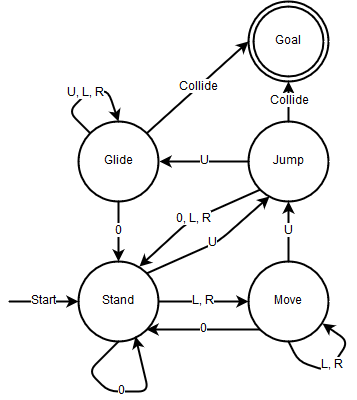
\includegraphics[width=0.5\textwidth]{fsa}
\caption{The FSA as a directed graph}
\end{figure}

\cprotect\sol{\\
  $A       = \{\Sigma, S, S_0, G, \delta\}$\\
  $\Sigma  = \{U, L, R, U, Collide\}$\\
  $S       = \{Stand, Move, Jump, Glide, Goal\}$\\
  $S_0     = Stand$\\
  $G       = \{Goal\}$\\
  $\delta  = $ \begin{tabular}{l|ccccc}
    & Stand & Move & Jump & Glide & Goal \\
    \hline
    0 & Stand & Stand & Stand & Stand & ?\\
    L & Move & Move & Stand & Glide & ? \\
    R & Move & Move & Stand & Glide & ? \\
    U & Jump & Jump & Glide & Glide & ? \\
    Collide & ? & ? & Goal & Goal & ?
  \end{tabular}
}

\FloatBarrier

\section{Old MacDonald Had A Farm}
Most of you will be familiar with the classic nursery rhyme of Old MacDonald and his farm full of animals. The first verse goes like this:\\\\
\textit{Old MacDonald had a farm, E-I-E-I-O\\
And on his farm he had a cow, E-I-E-I-O\\
With a moo-moo here and a moo-moo there\\
Here a moo\\
There a moo\\
Everywhere a moo-moo\\
Old MacDonald had a farm, E-I-E-I-O\\
}

\noindent In all subsequent verses, the next animal is introduced making its respective sound.\\
In the file \texttt{old\_macdonald.py}, you will find a function that reads this first verse out of a file named \texttt{old\_macdonald.txt}. Open the code and execute the script to look at the output.

\subsection{Old MacDonald's Cat}
Old MacDonald recently also got a cat, which unfortunately could not keep quiet and kept on meowing through the verse, which you will have seen in the output.\\
Each "meow" starts with either an uppercase or lowercase \textit{M}/\textit{m}, is followed by at least one \textit{e}, at least one \textit{o} and ends with exactly one \textit{w}.\\

\noindent Examples:\\
\textit{Meow\\
meeooow\\
Meeeeeeeeeeeow\\}

\noindent The code includes another function  \texttt{delete\_meow}. Right now it does nothing and only returns the same verse as it was given.\\
Modify the function such that it returns an altered version of the given verse in which each meowing following the exact described pattern is deleted. The function \texttt{sub} of the \texttt{re} module might be helpful.

\cprotect\sol{
\begin{python}
  def delete_meow(verse):
      """Deletes all the versions of cat noise from the input string."""
      return re.sub("(m|M)(e)+(o)+w",'',verse)
\end{python}
}

\subsection{Old MacDonald's Whole Farm}
Now let's sing the whole song!\\
First there is the cow going 'moo'.\\
Then a duck going 'quack'.\\
Then a horse going 'neigh'.\\
Then a pig going 'oink'.\\
And finally the cat, which can now go 'meow' after having waited its turn.\\
So, for example, the second verse looks like this:\\\\
\textit{
Old MacDonald had a farm, E-I-E-I-O\\
And on his farm he had a duck, E-I-E-I-O\\
With a quack-quack here and a quack-quack there\\
Here a quack\\
There a quack\\
Everywhere a quack-quack\\
Old MacDonald had a farm, E-I-E-I-O\\
}

\noindent Modify the given function  \texttt{sing\_song} to sing the song with all these animals (instead of only printing the first verse, as it does now)!\\\\
This is done easiest using string formatting:\\
\begin{description}
  \item - First, find the words "cow" and "moo" in the cat-free verse and replace them with formatting markers
  \item - Now use \texttt{.format()} to print the verse once for each animal with its respective sound and an empty line afterwards
  \item - Tip: You can create a compact and flexible solution by making a loop that prints each verse and saving all the animals and sounds in a collection as introduced last week.
\end{description}

\cprotect\sol{
\begin{python}
  def sing_song(verse):
      """
      Sings the song.
      
      Replacing all default "moo"s and "cow"s with formatting markers to then
      iterate over a list of animal-sound tuples and fill those markers in.
      """
      verse_rep = re.sub('cow','{0}', verse)
      verse_rep = re.sub('moo','{1}', verse_rep)
      # alternatively to re.sub, we can use
      # `verse.replace('cow','{0}').replace('moo','{1}')`
      # replace might be more suitable since we don't need regex

      animals = [
          ('cow','moo'),
          ('duck','quack'),
          ('horse','neigh'),
          ('pig','oink'),
          ('cat','meow')
        ]

      for animal in animals:
          print(verse_rep.format(animal[0],animal[1]),'\n')
\end{python}
}

\end{document}
